% D

% module Chapters.Chapter4.Example2 where

% E

\section{Example 2. Multiplication Table}
\label{sec:ex2}

The \clerk library supported connections between cells, tables, and sheets via reference offsets. In other words, the library allowed to set the relative positions of objects in a spreadsheet.

In this section, I described a spreadsheet with a multiplication table to demonstrate the connections between tables within a sheet.

The \cref{example2:tableValues} shows the resulting multiplication table and the \cref{example2:tableFormulas} shows the formulas inside that table.

\begin{figure}[h]
  \centering
  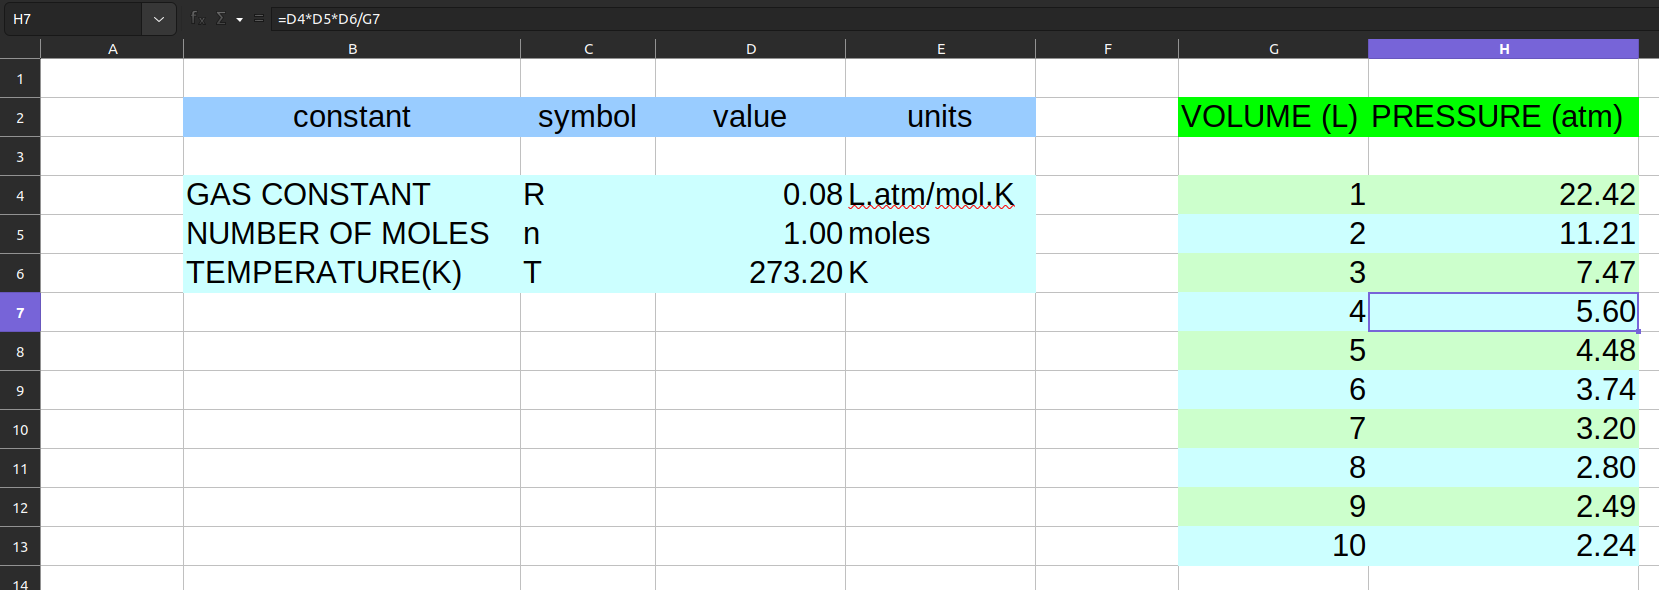
\includegraphics[scale=0.3]{demoValues.png}
  \caption{Multiplication table}
  \label{example2:tableValues}
\end{figure}

\begin{figure}[h]
  \centering
  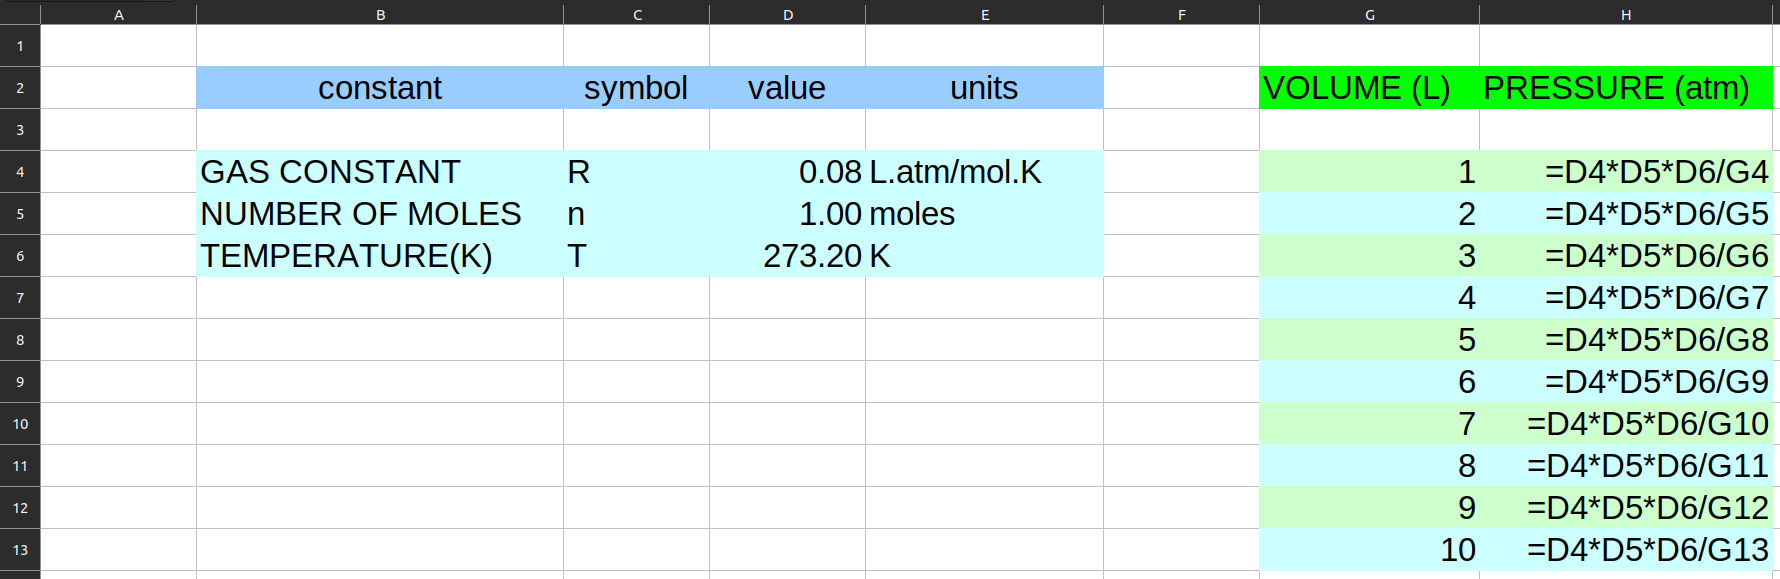
\includegraphics[scale=0.3]{demoFormulas.png}
  \caption{Multiplication table with formulas}
  \label{example2:tableFormulas}
\end{figure}

\subsection{Language Extensions}

First, I enabled the extension that simplified the work with string literals.

\begin{listing}[!h]
  \begin{minted}{haskell}
  {-# LANGUAGE OverloadedStrings #-}
\end{minted}
  \caption{Language extensions}
  \label{example2:languageExtensions}
\end{listing}

\subsection{Imports}

Then, I imported the necessary modules.
Here, I included \hs{Control.Monad} as the task required performing repetitive monadic actions.
The module \hs{Data.Text} was used for constructing sheet names.
The \hs{Lens.Micro} module provided optics for working with cell references.

\begin{listing}[!h]
  \begin{minted}{haskell}
  import Clerk
  import Control.Monad (forM, forM_, void)
  import qualified Data.Text as T
  import Lens.Micro ((&), (+~), (^.))
\end{minted}
  \caption{Imports}
  \label{example2:imports}
\end{listing}

\subsection{Tables}

\newcommand{\vh}{Vertical Header}
\newcommand{\hh}{Horizontal Header}

In my case, a table was a logically grouped set of cell references.
Each table should contain at least a single cell.
The tables that I constructed were the following:

\begin{itemize}
  \item A column with row numbers ("\vh");
  \item A row with column numbers ("\hh");
  \item Tables with results of multiplication of the numbers from these headers ("Inner Table").
\end{itemize}

\subsubsection{\vh}
\label{example2:verticalHeaderSection}

I planned to build a \vh as in \cref{example2:verticalHeader}.

\begin{figure}[h]
  \centering
  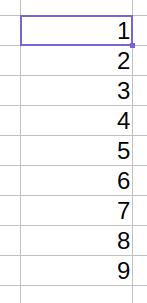
\includegraphics[scale=0.3]{vertical.png}
  \caption{\vh}
  \label{example2:verticalHeader}
\end{figure}

To achieve this goal, I had used the \clerk monadic interface to constructing rows and setting their positions within a sheet.

One of the monads provided by \clerk was the \hs{RowI} monad. Its name meant that inside that monad, I had to use a projection function from an \hs{input} type to \hs{CellData} type. The \hs{CellData} type was the type of spreadsheet values.

The effect of the \hs{RowI} monad was writing a template of a horizontal block of cells. The values obtained from \hs{input} via the projection function were placed onto a sheet according to that template.

I used the monadic function \hs{columnF} for constructing a \hs{RowI}. This function:
\begin{itemize}
  \item added a projected value into the template;
  \item added the formatting to the template;
  \item shifted a pointer to the next free cell in a template.
\end{itemize}

A vertical header contained just a single cell in each its row (\cref{example2:verticalHeader}). Such a header could be represented as several rows with verticall offset equal to \hs{1}. So, the rows were below each other.

I used a \hs{RowI} with one integer as an \hs{input} for a single row cell. This input was the index of the row within the \vh. I set the cell formatting to \hs{blank} since I did not need styling. I placed the rows for each input value onto a \hs{Sheet} and collected the references.

The placement of rows depended on input reference \hs{ref}. I could shift the rows within a sheet by varying this reference. Additionally, I decided to shift all rows vertically by \hs{2} from the input reference.

That said, the function \hs{mkVertical} (\cref{example2:verticalHeaderCode}) for each number from a given range of numbers (size of the multiplication table) and for each index of such a number runs a monadic function in the \hs{Sheet} monad via \hs{forM}. This function \hs{placeIn} at \hs{ref} shifted by \hs{index + 2} vertically places a number according to a \hs{RowI} produced by \hs{columnF}. \hs{columnF} makes a blank cell and uses a constant function as a projection function from the \hs{input} type of \hs{RowI} which is \hs{Int} in this case.

\begin{listing}[!h]
  \begin{minted}{haskell}
mkVertical :: Ref () -> [Int] -> Sheet [Ref Int]
mkVertical ref numbers =
  forM (zip [0 ..] numbers) $ \(idx, number) ->
    placeIn
    (ref & row +~ idx + 2)
    number
    ((columnF blank (const number)) :: RowI Int (Ref Int))
\end{minted}
  \caption{\vh}
  \label{example2:verticalHeaderCode}
\end{listing}

\subsubsection{\hh}
\label{example2:horizontalHeaderSection}

Next, I added a \hh (\Cref{example2:horizontalHeader}).

\begin{figure}[h]
  \centering
  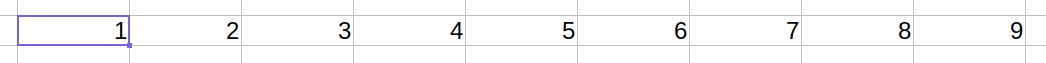
\includegraphics[scale=0.3]{horizontal.png}
  \caption{\hh}
  \label{example2:horizontalHeader}
\end{figure}

I made a row of numbers and collected the references to all its cells (\cref{example2:horizontalHeaderCode}). As the type of inputs was not important, I used the \hs{Row} type. This type assumed that the \hs{input} type was unit, or \hs{()}. In the \hs{Sheet} monad, I placed this row starting at a cell that was shifted horizontally by \hs{2} from the input reference. In this case, I used \hs{forM} to run the monadic function \hs{columnF} several times in the \hs{Row} monad.

\begin{listing}[!h]
  \begin{minted}{haskell}
mkHorizontal :: Ref () -> [Int] -> Sheet [Ref Int]
mkHorizontal ref numbers =
  place
  (ref & col +~ 2)
  ((forM numbers $ \n -> columnF blank (const n)) :: Row [Ref Int])
\end{minted}
  \caption{\hh}
  \label{example2:horizontalHeaderCode}
\end{listing}

\subsubsection{Inner Table}

The next step was to construct a table (\cref{example2:table}).

\begin{figure}[h]
  \centering
  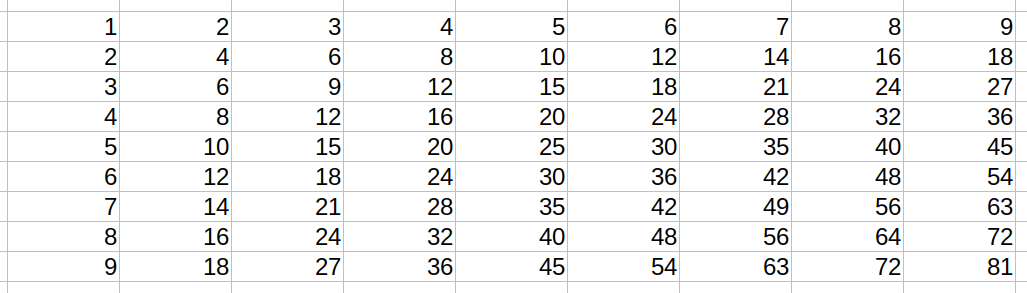
\includegraphics[scale=0.25]{table.png}
  \caption{Inner Table}
  \label{example2:table}
\end{figure}

The function \hs{mkTable} (\cref{example2:tableCode}) took a list of references to cells from the \vh and the \hh. For each such pair of references, it monadically made a coordinate via \hs{mkCoords}. This way, the \hs{mkCoords} function could access the current state of a \hs{Sheet}, e.g., its name and the workbook file path.

I decided to use single-cell rows for each Inner Table cell. This way, I could better align the positions of Inner Table cells with those of cells from headers. Moreover, I used the \hs{Row ()} type since I did not plan to use the references to table cells in other places.

The \hs{columnF} function used a projection to the formula \hs{r .* c}.
In other words, the reference to a cell from the \vh multiplied by the reference to a cell from the \hh.

\begin{listing}[!h]
  \begin{minted}{haskell}
mkTable :: [(Ref Int, Ref Int)] -> Sheet ()
mkTable cs =
  forM_ cs $ \(r, c) -> do
    coords <- mkCoords (c ^. col) (r ^. row)
    place coords ((columnF_ blank (const (r .* c))) :: Row ())  
\end{minted}
  \caption{Inner Table}
  \label{example2:tableCode}
\end{listing}

\subsection{Sheet}

Finally, I produced a complete \hs{Sheet ()}.
Here, I set the initial reference at \hs{B2}.
Then, I produced a list of numbers and constructed the headers.
Lastly, I used a list comprehension to generate all pairs of references to header cells and run \hs{mkTable} on this list of pairs.

\begin{listing}[!h]
  \begin{minted}{haskell}
sheet :: Sheet ()
sheet = do
  start <- mkRef' @"B2"
  let numbers = [1 .. 9]
  cs <- mkHorizontal start numbers
  rs <- mkVertical start numbers
  mkTable [(r, c) | r <- rs, c <- cs]
\end{minted}
  \caption{Inner Table}
  \label{example2:sheetCode}
\end{listing}

\subsection{Result}

To observe the resulting sheet, I run the \hs{main} function from \cref{example2:mainCode}.

\begin{listing}[!h]
  \begin{minted}{haskell}
main :: IO ()
main = writeXlsx "example2.xlsx" [(T.pack "List 1", void sheet)]
\end{minted}
  \caption{Writing result}
  \label{example2:mainCode}
\end{listing}

The resulting table looked as in \cref{example2:table}.